\documentclass[a4paper]{article}
\usepackage[a4paper,margin=0mm]{geometry}
\usepackage{fontspec}
\usepackage{unicode-math}
\usepackage{tikz}
\usepackage[table]{xcolor}
\usepackage[absolute]{textpos}
\usepackage{enumitem}
\usepackage{array}
\usepackage{multirow}

\setmainfont{Libertinus Serif}
\setsansfont{Libertinus Sans}
\setmathfont{Libertinus Math}
\newfontfamily\trackedsans{Libertinus Sans}[LetterSpace=8.0]

\definecolor{accent}{HTML}{602785}
\definecolor{badge}{HTML}{B8A0C8}
\definecolor{ink}{HTML}{2A2E30}

\setlength{\TPHorizModule}{1mm}
\setlength{\TPVertModule}{1mm}
\setlength{\parindent}{0pt}
\pagestyle{empty}

\newcommand{\LCOL}{16mm}
\newcommand{\RCOL}{111mm}
\newcommand{\COLW}{83mm}

\newcommand{\topicheader}[2]{%
\begin{textblock*}{194mm}(16mm,10mm)
\begin{tikzpicture}
\node[fill=accent,text=white,font=\sffamily\bfseries\fontsize{13}{13}\selectfont,
      minimum width=9mm,minimum height=9mm,inner sep=0pt] at (4.5mm,-4.5mm) {#1};
\node[font=\sffamily\bfseries\fontsize{15}{16}\selectfont,text=ink,anchor=west] at (12mm,-4.5mm) {#2};
\end{tikzpicture}
\end{textblock*}
\begin{textblock*}{194mm}(16mm,22.5mm)

\begin{tikzpicture}
\fill[accent] (0,0) rectangle (194mm,0.5mm);
\end{tikzpicture}
\end{textblock*}
}

\newcommand{\pagefooter}[1]{%
\begin{textblock*}{194mm}(8mm,286.41mm)
  
\begin{tikzpicture}
    \fill[accent] (0,0) rectangle (194mm,0.6mm);
  \end{tikzpicture}
\end{textblock*}
\begin{textblock*}{63.59mm}(8mm,288.27mm)
  {\sffamily\bfseries\color{accent}\fontsize{13}{16}\selectfont SAT 1200+}
\end{textblock*}
\begin{textblock*}{10mm}(188mm,288.27mm)
  \centering{\sffamily\color{accent}\fontsize{14}{16}\selectfont #1}
\end{textblock*}
}

\newcommand{\colrule}[2]{%
\begin{textblock*}{1mm}(105mm,#1mm)
\begin{tikzpicture}
\draw[black!65,line width=0.5pt] (0,0) -- (0,#2mm);
\end{tikzpicture}
\end{textblock*}
}

\newcommand{\setkicker}[2]{%
{\sffamily\bfseries\fontsize{12}{14}\selectfont #1.}\ {\itshape\fontsize{11}{14}\selectfont\color{black!75} #2}\par\vspace{2mm}%
}

\setlength{\fboxsep}{1.4pt}
\setlength{\fboxrule}{0.5pt}
\newcommand{\pnum}[1]{\fcolorbox{ink}{white}{\sffamily\bfseries\fontsize{8}{8}\selectfont #1}~}

\newcommand{\qrbox}[1]{%
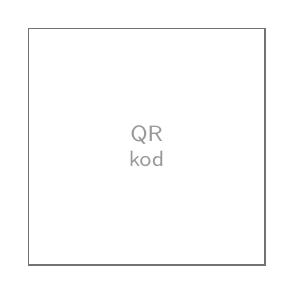
\begin{tikzpicture}
\draw[black!55,line width=0.6pt] (0,0) rectangle (30mm,30mm);
\node[black!40,font=\sffamily\fontsize{8}{9}\selectfont,align=center] at (15mm,15mm) {QR\\kod};
\end{tikzpicture}\\[1.5mm]
{\sffamily\fontsize{9}{11}\selectfont\color{black!70} #1}%
}

\arrayrulecolor{accent}
\setlength{\arrayrulewidth}{0.7pt}
\renewcommand{\arraystretch}{1.35}
\newcommand{\anstitle}[1]{{\sffamily\bfseries\color{accent}\fontsize{11}{13}\selectfont #1}\\[1.3mm]}

\begin{document}

% ================= PAGE 1: Set 1 | Set 2 =================
\topicheader{11}{Funksiya kompozitsiyasi va transformatsiyasi}
\pagefooter{59}
\colrule{32}{238}
\mbox{}%

\begin{textblock*}{\COLW}(\LCOL,32mm)
{\fontsize{12}{15}\selectfont
\setkicker{1-to'plam}{Nuqtada kompozitsiyani hisoblang. $f(x)=3x-2$, $g(x)=x^2+1$, $h(x)=2x+5$.}

\noindent\pnum{1} $f(g(2))=$\\[24mm]
\noindent\pnum{2} $g(f(1))=$\\[24mm]
\noindent\pnum{3} $f(h(0))=$\\[24mm]
\noindent\pnum{4} $h(g(1))=$\\[24mm]
\noindent\pnum{5} $g(g(1))=$\\[24mm]
\noindent\pnum{6} $f(f(2))=$
}
\end{textblock*}

\begin{textblock*}{\COLW}(\RCOL,32mm)
{\fontsize{12}{15}\selectfont
\setkicker{2-to'plam}{Kompozitsiyani algebraik tarzda to'liq soddalashtiring.}

\noindent\pnum{1} $f(g(x))=$\\[24mm]
\noindent\pnum{2} $g(f(x))=$\\[24mm]
\noindent\pnum{3} $f(h(x))=$\\[24mm]
\noindent\pnum{4} $h(f(x))=$\\[24mm]
\noindent\pnum{5} $g(h(x))=$\\[24mm]
\noindent\pnum{6} $h(g(x))=$
}
\end{textblock*}

\clearpage

% ================= PAGE 2: Set 3 | Set 4 =================
\topicheader{11}{Funksiya kompozitsiyasi va transformatsiyasi}
\pagefooter{60}
\colrule{32}{238}
\mbox{}%

\begin{textblock*}{\COLW}(\LCOL,32mm)
{\fontsize{12}{15}\selectfont
\setkicker{3-to'plam}{Vertikal transformatsiya. $f(x)=x^2-4$.}

\noindent\pnum{1} $f(3)+5=$\\[22mm]
\noindent\pnum{2} $f(1)-3=$\\[22mm]
\noindent\pnum{3} $-f(2)=$\\[22mm]
\noindent\pnum{4} $2f(1)=$\\[22mm]
\noindent\pnum{5} $-f(0)+1=$\\[22mm]
\noindent\pnum{6} $f(4)=\,?$ va $f(4)+2=\,?$ Natija qancha siljidi?
}
\end{textblock*}

\begin{textblock*}{\COLW}(\RCOL,32mm)
{\fontsize{12}{15}\selectfont
\setkicker{4-to'plam}{Gorizontal transformatsiya (ishora qopqoni). $f(x)=x^2-4$.}

\noindent\pnum{1} $f(x-3)$ da $x=5$\\[22mm]
\noindent\pnum{2} $f(x+2)$ da $x=1$\\[22mm]
\noindent\pnum{3} $f(-x)$ da $x=3$\\[22mm]
\noindent\pnum{4} $f(x-1)$ da $x=0$\\[22mm]
\noindent\pnum{5} $f(x-2)$ da $x=6$ va $f(x)$ da $x=4$. Nimani sezdingiz?\\[8mm]
\noindent\pnum{6} $f(-x)$ da $x=-2$
}
\end{textblock*}

\clearpage

% ================= PAGE 3: Set 5 | Set 6 (spot the error) =================
\topicheader{11}{Funksiya kompozitsiyasi va transformatsiyasi}
\pagefooter{61}
\colrule{32}{238}
\mbox{}%

\begin{textblock*}{\COLW}(\LCOL,32mm)
{\fontsize{11.5}{14.5}\selectfont
\setkicker{5-to'plam}{Aralash -- kompozitsiya va transformatsiya birgalikda.}

\noindent\pnum{1} $f(x)=x^2+1$, $g(x)=x-3$. $f(g(x))=\,?$, $x=5$ da qiymati?\\[12mm]
\noindent\pnum{2} $f(x)=2x+3$. $f(x-1)$ ni $x=4$ da baholang.\\[14mm]
\noindent\pnum{3} $g(x)=x^2-2x$. $g(-x)$ ni soddalashtiring.\\[12mm]
\noindent\pnum{4} $f(x)=x^2+1$, $g(x)=x+2$. $g(f(2))=\,?$\\[12mm]
\noindent\pnum{5} $f(x)=x^2-5$. $-f(x-1)$ ni $x=3$ da baholang.\\[12mm]
\noindent\pnum{6} $f(x)=3x$. $f(f(2))=\,?$
}
\end{textblock*}

\begin{textblock*}{\COLW}(\RCOL,32mm)
{\fontsize{10.3}{13}\selectfont
\setkicker{6-to'plam}{Xatoni toping -- buzilgan qadamni ayting, to'g'ri javobni bering.}

\noindent\pnum{1} $f(x)=x^2+1$, $g(x)=2x$. $f(g(3))$ ni toping:\\[1mm]
\hspace*{7mm}\textit{``$f(3)=10$, so'ngra $g(10)=20$.''}\\[2mm]
\hspace*{7mm}Xato va to'g'ri javob: \makebox[52mm]{\dotfill}\\[6mm]

\noindent\pnum{2} $f(x)=x^2-4$. $f(3)+2$ ni toping:\\[1mm]
\hspace*{7mm}\textit{``$f(x+2)$ ni hisoblaymiz: $f(5)=21$.''}\\[2mm]
\hspace*{7mm}Xato va to'g'ri javob: \makebox[52mm]{\dotfill}\\[6mm]

\noindent\pnum{3} $f(x)=x^2+3x$. $f(x-2)$ ni $x=5$ da toping:\\[1mm]
\hspace*{7mm}\textit{``Chapga siljiydi: $f(x+2)=f(7)=70$.''}\\[2mm]
\hspace*{7mm}Xato va to'g'ri javob: \makebox[52mm]{\dotfill}\\[6mm]

\noindent\pnum{4} $f(x)=x^2-1$. $f(-x)$ ni $x=2$ da toping:\\[1mm]
\hspace*{7mm}\textit{``$f(-x)=-f(x)$, shuning uchun $-f(2)=-3$.''}\\[2mm]
\hspace*{7mm}Xato va to'g'ri javob: \makebox[52mm]{\dotfill}\\[6mm]

\noindent\pnum{5} $f(x)=2x+1$, $g(x)=x-4$. $g(f(x))$ ni toping:\\[1mm]
\hspace*{7mm}\textit{``$f(g(x))=2(x-4)+1=2x-7$.''}\\[2mm]
\hspace*{7mm}Xato va to'g'ri javob: \makebox[52mm]{\dotfill}
}
\end{textblock*}

\clearpage

% ================= PAGE 4: Set 7 (bonus) =================
\topicheader{11}{Funksiya kompozitsiyasi va transformatsiyasi}
\pagefooter{62}
\colrule{32}{238}
\mbox{}%

\begin{textblock*}{\COLW}(\LCOL,32mm)
{\fontsize{12}{15}\selectfont
\setkicker{7-to'plam}{Bonus / qiyin.}

\noindent\pnum{1} $f(x)=x^2-2x+1$, $g(x)=x+3$. $f(g(x))$ ni to'liq soddalashtiring.\\[16mm]
\noindent\pnum{2} $f(x)=x^2-4$. $-f(x-1)$ ni $x=0$ da baholang.\\[22mm]
\noindent\pnum{3} $f(x)=2x-5$, $g(x)=x^2+1$. $g(f(2))$ va $f(g(2))$ ni toping -- teng me?\\[22mm]
\noindent\pnum{4} $f(x)=x^2+1$. $h(x)=f(x-3)+2$ bo'lsa, $h(5)$ ni toping.\\[22mm]
\noindent\pnum{5} $f(x)=3x+2$. $f(f(x))$ ni soddalashtiring.
}
\end{textblock*}

\clearpage

% ================= PAGE 5: Javoblar =================
\topicheader{11}{Funksiya kompozitsiyasi va transformatsiyasi}
\pagefooter{63}
\mbox{}%

\begin{textblock*}{194mm}(16mm,30mm)
{\bfseries\itshape\color{accent}\fontsize{19}{21}\selectfont\centering Javoblar\par}
\end{textblock*}

\begin{textblock*}{194mm}(16mm,44mm)
{\fontsize{9.3}{11.8}\selectfont
\centering
\renewcommand{\arraystretch}{1.3}
\begin{tabular}{|>{\centering\arraybackslash}p{24mm}|>{\centering\arraybackslash}p{9mm}|>{\centering\arraybackslash}p{34mm}|>{\centering\arraybackslash}p{9mm}|>{\centering\arraybackslash}p{34mm}|}
\hline
\rowcolor{badge!55}\textbf{To'plam} & \textbf{\#} & \textbf{Javob} & \textbf{\#} & \textbf{Javob}\\
\hline
\multirow{3}{24mm}{\centering 1-to'plam} & 1 & 13 & 2 & 2\\\cline{2-5}
 & 3 & 13 & 4 & 9\\\cline{2-5}
 & 5 & 5 & 6 & 10\\\hline
\multirow{3}{24mm}{\centering 2-to'plam} & 1 & $3x^2+1$ & 2 & $9x^2-12x+5$\\\cline{2-5}
 & 3 & $6x+13$ & 4 & $6x+1$\\\cline{2-5}
 & 5 & $4x^2+20x+26$ & 6 & $2x^2+7$\\\hline
\multirow{3}{24mm}{\centering 3-to'plam} & 1 & 10 & 2 & $-6$\\\cline{2-5}
 & 3 & 0 & 4 & $-6$\\\cline{2-5}
 & 5 & 5 & 6 & \multicolumn{1}{p{34mm}|}{\centering $f(4)\!=\!12$, $+2\!=\!14$}\\\hline
\multirow{3}{24mm}{\centering 4-to'plam} & 1 & 0 & 2 & 5\\\cline{2-5}
 & 3 & 5 & 4 & $-3$\\\cline{2-5}
 & 5 & \multicolumn{1}{p{34mm}|}{\centering teng, $=12$} & 6 & 0\\\hline
\multirow{3}{24mm}{\centering 5-to'plam} & 1 & $x^2{-}6x{+}10$; $5$ & 2 & 9\\\cline{2-5}
 & 3 & $x^2+2x$ & 4 & 7\\\cline{2-5}
 & 5 & 1 & 6 & 18\\\hline
\multirow{3}{24mm}{\centering 7-to'plam} & 1 & $x^2+4x+4$ & 2 & 3\\\cline{2-5}
 & 3 & \multicolumn{1}{p{34mm}|}{\centering $2$, $5$ -- teng emas} & 4 & 7\\\cline{2-5}
 & 5 & $9x+8$ & -- & --\\\hline
\multirow{5}{24mm}{\centering 6-to'plam} & \multicolumn{4}{p{86mm}|}{1.\ Kompozitsiya tartibi teskari olingan ($g(f(3))$ emas, $f(g(3))$ kerak). To'g'ri: $g(3)=6$, $f(6)=37$.}\\\cline{2-5}
 & \multicolumn{4}{p{86mm}|}{2.\ $f(x)+2$ (natijaga qo'shish) bilan $f(x+2)$ (kirishga qo'shish) aralashtirilgan. To'g'ri: $f(3)=5$, $f(3)+2=7$.}\\\cline{2-5}
 & \multicolumn{4}{p{86mm}|}{3.\ $f(x-h)$ o'ngga siljiydi deb noto'g'ri faraz qilingan. To'g'ri: $f(3)=18$.}\\\cline{2-5}
 & \multicolumn{4}{p{86mm}|}{4.\ $f(-x)=-f(x)$ deb noto'g'ri faraz qilingan. To'g'ri: $f(-2)=3$.}\\\cline{2-5}
 & \multicolumn{4}{p{86mm}|}{5.\ So'ralgan $g(f(x))$ o'rniga $f(g(x))$ hisoblangan. To'g'ri: $g(f(x))=2x-3$.}\\\hline
\end{tabular}
}
\end{textblock*}

\begin{textblock*}{194mm}(16mm,252mm)
\centering
{\sffamily\fontsize{9.5}{11.5}\selectfont\color{black!70} Video yechimlar va qo'shimcha testlar uchun quyidagi QR kodlarni skanerlang:}\\[4mm]
\begin{minipage}[t]{32mm}\centering\qrbox{YouTube}\end{minipage}%
\hspace{16mm}%
\begin{minipage}[t]{32mm}\centering\qrbox{Telegram}\end{minipage}
\end{textblock*}

\end{document}
